\documentclass{article}
\usepackage{latexsym, epsfig, amsmath, amssymb, amsfonts}



\usepackage{tkz-euclide}
\usepackage{pgfplots}
\usepackage{tikz}


%\usetikzlibrary{
%	plotmarks,patterns
%	,decorations.shapes
%	,decorations.text
%	,decorations.footprints
%	,decorations.fractals
%	,decorations.pathmorphing
%	,shadows
%	,matrix
%	,positioning
%	,fadings
%}
%\pgfplotsset{compat=1.11}


%\newcommand{\F}{\mathcal{F}}
\pagenumbering{gobble}

\begin{document}
\begin{figure}[htbb]
\begin{center}
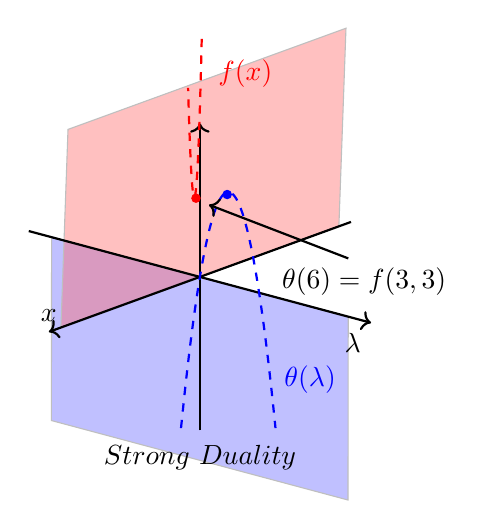
\begin{tikzpicture}%[scale=1.0]
\fill[blue!62,opacity=0.4,rotate=-15,scale=1.5] (-1.3,0,0) -- (1.3,0,0) -- (1.7,-1.5,0) -- (-0.9,-1.5,0) -- (-1.3,0,0);
\draw[lightgray,rotate=-15,scale=1.5] (-1.3,0,0) -- (1.3,0,0) -- (1.7,-1.5,0) -- (-0.9,-1.5,0) -- (-1.3,0,0);
\fill[red!62,opacity=0.4,rotate=-25,scale=1.5] (0,0,-2.3) -- (0,0,2.3) -- (0,2.2,4) -- (0,2.2,-0.6) -- (0,0,-2.3);
\draw[lightgray,rotate=-25,scale=1.5] (0,0,-2.3) -- (0,0,2.3) -- (0,2.2,4) -- (0,2.2,-0.6) -- (0,0,-2.3);
\draw[thick,->,rotate=-15,scale=1.5] (-1.5,0,0) -- (1.5,0,0) node[anchor=north east]{$\lambda$};
\draw[thick,->,scale=1.5] (0,-1.3,0) -- (0,1.3,0);% node[anchor=north west]{$z$};
\draw[thick,->,rotate=-25,scale=1.5] (0,0,-2.5) -- (0,0,2.5) node[anchor=south]{$x$};
\draw[domain=-1:6.5, smooth, variable=\x, red,thick,dashed,scale=0.06] plot (0, {2*(\x-3)*(\x-3)+18},{\x});
\draw[domain=-4:16, smooth, variable=\x, blue,thick,dashed,scale=0.06] plot (\x, {6*\x-(0.5*\x*\x)},0);
\filldraw[red] (-0.05,1,0) circle (1.5pt);
\filldraw[blue] (0,0.7,-0.9) circle (1.5pt);\node[red] at (0,2,-1.5) {$f(x)$};\node[blue] at (1.4,-1.3,0) {$\theta(\lambda)$};
\draw[->,black,thick] (1.5,-0.15,-1) -- (0,0.8,-0.3);\node[black] at (1.7,-0.45,-1) {$\theta(6) = f(3,3)$};
\node[black] at (0,-2.3,0) {$Strong~Duality$};
\end{tikzpicture}
\end{center}
\end{figure}

\end{document}